\documentclass[tikz]{standalone}
    \usepackage{tikz}
    \usetikzlibrary{positioning, graphs}
    \usetikzlibrary{graphs.standard}
    \begin{document}
    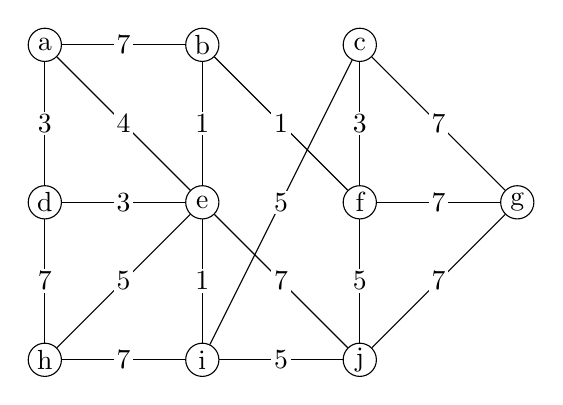
\begin{tikzpicture}
    \begin{scope}
        [vertex/.style={draw,circle,inner sep = 0em, minimum size = 1.2em},
            edgelabel/.style = {fill = white, inner sep = 0.1em}]
        \node[vertex] (a) at (0,0) {a};
        \node[vertex] (b) at (2,0) {b};
        \node[vertex] (c) at (4,0) {c};
        \node[vertex] (d) at (0,-2) {d};
        \node[vertex] (e) at (2,-2) {e};
        \node[vertex] (f) at (4,-2) {f};
        \node[vertex] (g) at (6,-2) {g};
        \node[vertex] (h) at (0,-4) {h};
        \node[vertex] (i) at (2,-4) {i};
        \node[vertex] (j) at (4,-4) {j};
        
        \draw[-] (a) to node[edgelabel]{$7$} (b);
        \draw[-] (a) to node[edgelabel]{$3$} (d);
        \draw[-] (a) to node[edgelabel]{$4$} (e);
        \draw[-] (b) to node[edgelabel]{$1$} (e);
        \draw[-] (b) to node[edgelabel]{$1$} (f);
        \draw[-] (c) to node[edgelabel]{$3$} (f);
        \draw[-] (c) to node[edgelabel]{$7$} (g);
        \draw[-] (c) to node[edgelabel]{$5$} (i);
        \draw[-] (d) to node[edgelabel]{$3$} (e);
        \draw[-] (d) to node[edgelabel]{$7$} (h);
        \draw[-] (e) to node[edgelabel]{$5$} (h);
        \draw[-] (e) to node[edgelabel]{$1$} (i);
        \draw[-] (e) to node[edgelabel]{$7$} (j);
        \draw[-] (f) to node[edgelabel]{$7$} (g);
        \draw[-] (f) to node[edgelabel]{$5$} (j);
        \draw[-] (g) to node[edgelabel]{$7$} (j);
        \draw[-] (h) to node[edgelabel]{$7$} (i);
        \draw[-] (i) to node[edgelabel]{$5$} (j);
    \end{scope}
    \end{tikzpicture}
    \end{document}